\chapter{Proposed Methodology and System Design} \label{Methodology} 

\section{Motivation}
Nowadays, healthcare systems are overwhelmed with patients who have to be monitored continuously because of their chronic conditions, postoperative situations, or remote living. Hospitals equipped with conventional monitoring devices are not only time-consuming and costly but also impractical for long-term monitoring. Given the developments in IoT and cloud computing, Remote Patient Monitoring (RPM) offers the possibility of real-time health data acquisition from patients and direct data transfer to doctors or hospitals. On the other hand, the biggest issue that security and privacy concerns regarding the medical data being transmitted.

Most of the present IoT-based solutions have either password-based or RSA-based authentication mechanisms, which can be weak or computationally expensive for small devices such as Arduino or ESP modules. Hence, this project is arisen from the demand for a healthcare data privacy ensuring, third-party access denial preventing, and patient authentication process confidential and secure yet lightweight, resistant to the security threats, and reliable in performance problem.

Therefore, the solution integrates Elliptic Curve Cryptography (ECC) for lightweight encryption, blockchain technology for secure and tamper-proof record management, and a cloud-based system to facilitate easy real-time access by the doctors.

\section{System Architecture}
The proposed system is a combination of IoT devices, cloud storage, and blockchain-based security. It can be divided into four primary layers as illustrated in Fig. \ref{fig:system_architecture}.

\begin{figure}[H]
    \centering
    \includegraphics[width=1.0\textwidth]{Chap02/layers.png}
    \caption{System Architecture of Remote Patient Monitoring}
    \label{fig:system_architecture}
\end{figure}

\subsection{Patient Layer (Device Layer)}
The patient layer comprises physiological sensors including the Temperature Sensor (LM35) and Pulse Oximeter (MAX30100) that monitor vital health parameters. These sensors are interfaced with an Arduino UNO microcontroller that gathers real-time health data from the patient. The encrypted data is then transmitted to the cloud platform through an ESP8266 Wi-Fi module, ensuring secure wireless communication.

\subsection{Network / Cloud Layer}
The ThingSpeak IoT Cloud Platform is utilized for storing and receiving patient data in real-time. All transmitted information is maintained in an encrypted format using the session key generated via ECC. Before accepting any incoming data, the blockchain layer verifies the authenticity of the sender (patient's device) to ensure that only legitimate devices can upload health information to the cloud.

\subsection{Blockchain Authentication Layer}
Every enrolled patient device is provisioned with a digital smart card containing authentication credentials. These smart cards are registered in the blockchain ledger, which provides high security and prevents unauthorized alterations. During each connection attempt, a mutual authentication process occurs between the patient device, cloud server, and hospital server. If the verification fails at any stage, the connection request is denied, preventing unauthorized access to the system.

\subsection{Hospital Server and Doctor Layer}
The hospital server validates the incoming information from the blockchain through a secure dashboard interface. Authorized doctors can access the patient's real-time health status through this server and intervene promptly if any abnormality is detected in the vital signs.

\section{Working Flow}

% \begin{figure}[H]
%     \centering
%     \includegraphics[width=0.9\textwidth]{Chap02/workflow.png}
%     \caption{System Workflow: Registration, Authentication, Data Transmission, and Monitoring}
%     \label{fig:workflow}
% \end{figure}

The complete system workflow consists of six major phases. Initially, during patient registration, the patient's device is registered with the hospital server, where a smart card containing cryptographic parameters is generated and its hash is saved on the blockchain. In the data collection phase, the sensors continuously measure the vital signs of the patient including temperature and SpO₂ levels, and forward this data to the Arduino microcontroller.

The data encryption phase involves the implementation of ECC by the Arduino to encode the collected data using the session key (SK). Subsequently, during data transmission, the encrypted data is transferred to the ThingSpeak Cloud through the Wi-Fi module. The authentication and verification phase ensures that the blockchain performs a comprehensive check between the device credentials and the stored records; if the verification is successful, the data is accepted into the system. Finally, in the data access phase, the verified data is retrieved by the hospital server, enabling doctors to remotely monitor and follow up with patients from any location.

\section{Algorithm Explanation}
The presented scheme is a simplified, lightweight, blockchain-enabled authentication version adapted from the Internet of Drones paper \cite{1}, which forms the basis for this system. The algorithm operates in three distinct phases as depicted in Fig. \ref{fig:algo_diagram}.

\subsection{Phase 1: Registration}
During the registration phase, the hospital server initializes the elliptic curve parameters and establishes the cryptographic infrastructure. The patient device submits its identity and password credentials to the server. Upon verification, the server generates a smart card embedded with the necessary cryptographic parameters and stores its hash on the blockchain for future authentication. The patient receives this smart card which contains the public parameters required for subsequent secure communications.

\subsection{Phase 2: Authentication}
The authentication phase begins when the patient device uses the smart card to initiate a login session. Both the device and the server generate random nonces, and ECC operations are performed to derive the shared session key (SK). Ethereum smart contracts are employed to validate the identities of all participating entities and prevent impersonation attacks. Upon successful completion of all verification steps, the communicating parties establish a secure encrypted channel for data exchange.

\subsection{Phase 3: Data Transmission}
In the data transmission phase, the Arduino microcontroller encrypts the patient's health data using the established session key. The encrypted data is then securely transmitted to the cloud platform through the wireless network. At the receiving end, the hospital server decrypts the data using the same session key, making it available for authorized medical personnel to view and analyze.

\begin{figure}[H]
    \centering
    \includegraphics[width=0.98\textwidth]{Chap02/flowDiagram.png}
    \caption{Algorithm Flow Diagram}
    \label{fig:algo_diagram}
\end{figure}

\section{Hardware Components}

The system integrates multiple hardware modules to achieve reliable physiological signal acquisition, processing, and wireless communication. The key components include the ESP32 DevKit V1 (DOIT), MAX30100 pulse oximeter and heart-rate sensor, power interfaces, and optional controller variants. Each component and its connectivity are detailed below.

\subsection{ESP32 DevKit V1 (DOIT)}

The ESP32 DevKit V1 (DOIT) serves as the primary compute and communication module. It provides an enable (EN) pin, VIN, 3V3 output, and multiple ADC-capable GPIOs. The board supports UART0 and UART2 (TX0/RX0, TX2/RX2) and I\textsuperscript{2}C communication via pins D21 (SDA) and D22 (SCL) for sensor interfacing.  
It exposes general-purpose pins D23, D22, D21, D19, D18, D5, D4, D2, D15, and D13, along with ground and power rails clearly marked on the PCB silkscreen.  
The integrated USB interface enables both power supply and firmware programming, while the Boot and Enable buttons facilitate flashing and runtime control of the module.

\subsection{MAX30100 Pulse Oximeter and Heart-Rate Sensor}

The MAX30100 sensor integrates dual LEDs and photodiodes for simultaneous measurement of heart rate and blood oxygen saturation (SpO\textsubscript{2}).  
Its pin configuration includes VIN, SCL, SDA, INT, IRD/RD, and GND. The device operates through an I\textsuperscript{2}C interface connected to the ESP32 for data acquisition.  
In the schematic representation, the MAX30100 is shown as a 7-pin block connected to the I\textsuperscript{2}C network and ground. This configuration ensures stable communication and accurate physiological signal measurement.

\subsection{Power Interfaces}

A 2-pin screw terminal labeled \textbf{POWER} provides a stable external power input with a dedicated ground return.  
The ESP32 DevKit also exposes VIN and 3V3 rails through header pins, which are used to power the MAX30100 and any auxiliary modules.  
Proper grounding practices are followed across the MCU and sensor networks, indicated by multiple GND symbols in the schematic. This reduces electrical noise and ensures accurate analog readings during sensor operation.

\subsection{Optional Controller Variant}

An alternative schematic variant includes an Arduino Nano footprint with a complete pin map (A0–A7, D0–D13, 5V, 3V3, VIN), placed alongside the ESP32 DevKit.  
This configuration allows flexible prototyping and hybrid deployment scenarios.  
While the provided design connects the MAX30100 to the ESP32, the dual-MCU arrangement enables division of tasks—where the Nano can handle timing-critical sampling and the ESP32 can manage wireless connectivity and security operations.

\subsection{Board-Level Pinout Highlights}

The PCB legend lists the key pin references including EN, VIN, 3V3, GND, UARTs (TX0/RX0, TX2/RX2), and general-purpose I/O pins (D21–D27, D33–D39).  
These annotations simplify hardware assembly and firmware pin mapping during setup.  
The MAX30100 pads are grouped with a local ground reference to maintain clean signal routing.  
The comprehensive silkscreen details accelerate hardware bring-up and minimize wiring errors during sensor installation.

\begin{figure}[H]
    \centering
    \begin{subfigure}[b]{0.38\textwidth}
        \centering
        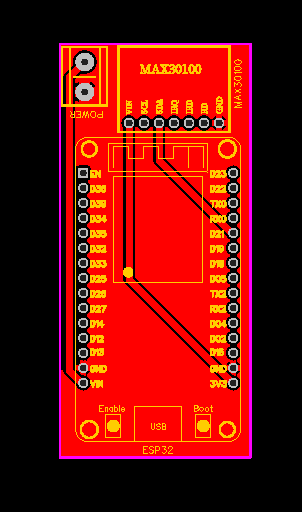
\includegraphics[width=\textwidth]{Chap02/PCB_PCB_IoT-project-copy_2025-11-10 (1).pdf}
        \caption{PCB Design - Bottom View}
        \label{fig:pcb_schematic_top}
    \end{subfigure}
    \hfill
    \begin{subfigure}[b]{0.38\textwidth}
        \centering
        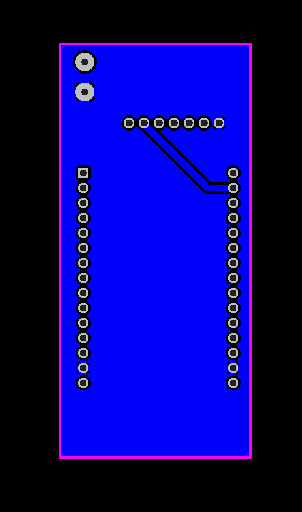
\includegraphics[width=\textwidth]{Chap02/PCB_PCB_IoT-project-copy_2025-11-10 (2).pdf}
        \caption{PCB Design - Top View}
        \label{fig:pcb_schematic_bottom}
    \end{subfigure}
    
    \vspace{0.5cm}
    
    \begin{subfigure}[b]{0.75\textwidth}
        \centering
        \includegraphics[width=\textwidth]{Chap02/WhatsApp Image 2025-11-11 at 4.13.36 PM.jpeg}
        \caption{PCB Schematic Diagram}
        \label{fig:pcb_schematic}
    \end{subfigure}
    \caption{PCB Design and Schematic}
    \label{fig:pcb_complete}
\end{figure}

\begin{figure}[H]
    \centering
    \begin{subfigure}[b]{0.48\textwidth}
        \centering
        \includegraphics[width=\textwidth]{Chap02/WhatsApp Image 2025-11-11 at 12.43.59 PM (1).jpeg}
        \caption{Circuit Layout}
        \label{fig:hardware_circuit}
    \end{subfigure}
    \hfill
    \begin{subfigure}[b]{0.48\textwidth}
        \centering
        \includegraphics[width=\textwidth]{Chap02/WhatsApp Image 2025-11-11 at 12.43.59 PM.jpeg}
        \caption{Physical Assembly}
        \label{fig:hardware_assembly}
    \end{subfigure}
    \caption{Hardware Implementation}
    \label{fig:hardware_implementation}
\end{figure}

\vspace{5.5cm}

\section{Mathematical Overview of ECC}

Elliptic Curve Cryptography (ECC) employs algebraic structures of elliptic curves that are defined over finite fields.
An elliptic curve $E$ over a finite field $\mathbb{F}_p$ (where $p$ is a large prime) can be described by the Weierstrass equation:
\begin{equation}
E: y^2 \equiv x^3 + ax + b \pmod{p}, \quad \text{with } 4a^3 + 27b^2 \not\equiv 0 \pmod{p}.
\end{equation}
The points $P = (x, y)$ that satisfy this equation together with the point at infinity $\mathcal{O}$ form an abelian group under point addition.

\subsection{Group Law on Elliptic Curves}
If $P = (x_1, y_1)$ and $Q = (x_2, y_2)$ are two different points on the curve $E$, then the addition operation $R = P + Q = (x_3, y_3)$ is given by:
\begin{equation}
\lambda = \frac{y_2 - y_1}{x_2 - x_1} \pmod{p}, \quad
x_3 = \lambda^2 - x_1 - x_2 \pmod{p}, \quad
y_3 = \lambda(x_1 - x_3) - y_1 \pmod{p}.
\end{equation}
If $P$ is equal to $Q$, then the doubling operation $R = 2P = (x_3, y_3)$ is expressed as:
\begin{equation}
\lambda = \frac{3x_1^2 + a}{2y_1} \pmod{p}, \quad
x_3 = \lambda^2 - 2x_1 \pmod{p}, \quad
y_3 = \lambda(x_1 - x_3) - y_1 \pmod{p}.
\end{equation}
The \textbf{scalar multiplication} which is basically repeated addition of a point, and thus related to ECC, can be written as:
\begin{equation}
Q = kP = \underbrace{P + P + \cdots + P}_{k \text{ times}}.
\end{equation}
From a computing viewpoint, it is extremely difficult to find $k$ if only $P$ and $Q = kP$ are given. This problem is termed the \textbf{Elliptic Curve Discrete Logarithm Problem (ECDLP)} and is the leading cause why ECC is secure.

\subsection{Key Generation}
In the patient monitoring system employing ESP32, the generation of private key $d$ and public key $Q$ for each device can be represented as the outcome of:
\begin{align}
\text{Private key: } & d \in [1, n-1], \\
\text{Public key: } & Q = dG,
\end{align}
where $G$ is a publicly known (shared) base point on $E$ of prime order $n$.
The public key $Q$ is the one that is given to the authentication server during device provisioning. The private key $d$ is, however, the one that remains with the secure device.

Every party has:
\begin{itemize}
    \item A private key (d)
    \item A public key (Q = d \times G), where G is a point on the curve.
\end{itemize}

The session key (SK) is generated by:
\[
    SK = (d_A \times Q_B) = (d_B \times Q_A)
\]
which allows both parties to have the same shared key without letting other parties know it.
This is the key that is utilized for encrypting the medical data before the data is sent to the cloud.

\subsection{Authentication Using ECC-based Challenge–Response}
To have an authentication mechanism secure enough between an ESP32 device and a cloud server, an ECC-based digital signature (ECDSA) is employed. 
The steps of the protocol are as follows:
\begin{enumerate}
 \item The server creates a random challenge message $m$ and sends it to the device.
 \item The device, receiving the message, calculates the hash $e = H(m)$ of $m$ using SHA-256.
 \item The device selects $k \in [1, n-1]$ at random, computes the point on the elliptic curve:
 \begin{equation}
 R = kG = (x_r, y_r),
 \end{equation}
 and then computes the signature components:
 \begin{align}
 r & = x_r \bmod n, \\
 s & = k^{-1}(e + dr) \bmod n.
 \end{align}
 The signature is $(r, s)$.
 \item The device sends to the server the signature $(r, s)$.
 \item The server, with the help of device's public key $Q = dG$, performs the operations below to validate the signature:
 \begin{align}
 w & = s^{-1} \bmod n, \\
 u_1 & = ew \bmod n, \quad u_2 = rw \bmod n, \\
 X & = u_1G + u_2Q = (x_v, y_v), \\
 v & = x_v \bmod n.
 \end{align}
If $v$ is equal to $r$, then the signature is correct, thus, the device is authenticated.
\end{enumerate}

\subsection{Mathematical Proof of Correctness}
Substituting $Q = dG$ and expanding the expression:
\begin{equation}
X = u_1G + u_2Q = (ew + rw d)G.
\end{equation}
Given that $w = s^{-1}$ and $s = k^{-1}(e + dr)$, the expression is:
\begin{align}
ew + rw d & = e s^{-1} + r s^{-1} d \\
&= e (k(e + dr)^{-1}) + r d (k(e + dr)^{-1}) \\
&= k^{-1} (e + dr)(e + dr)^{-1} = k^{-1}k = 1.
\end{align}
Or:
\begin{equation}
X = kG = R \implies v = r,
\end{equation}
which is the statement that the verification equation works for a valid signature.

\subsection{Integration into the Proposed RPM System}
The authentication with ECC in the remote patient monitoring (RPM) system that is the method by which only real ESP32 devices are allowed to send the patient's vital data to the cloud. The sequence of events is:
\begin{enumerate}
 \item An ECC key pair $(d, Q)$ is available for each ESP32 device.
 \item The server, after the link is set up, sends the device a nonce $m$ as a challenge.
 \item Signing $m$ by $d$ according to ECDSA steps given above is how the device makes use of his private key $d$.
 \item Checking the signature by the server using the public key $Q$ is the next step.
 \item Secure communication (TLS or session key) for the encrypted transfer of patient data is set up if everything is in order.
\end{enumerate}
This sort of a scheme is considerate of the security aspect while, at the same time, it bears very little computing power on the part of the ESP32. Switching to ECC from the conventional RSA means that both key size and computation time can be lowered significantly, thus, the limited capabilities of IoT devices in the healthcare sector can be dealt with.

\subsection{Security Strength}
The ECC model may provide the very same security standard as RSA, but the key sizes are considerably smaller. For instance:
\begin{equation}
\text{RSA-3072} \approx \text{ECC-256 in security strength.}
\end{equation}
As such, ECC can be used to securely provide authentication and data integrity without any detrimental effect on performance and power consumption of the device which in the case of ESP32 are quite limited.

\begin{table}[!ht]
    \centering
    \caption{System Stages, Components, and Purpose}
    \begin{tabular}{|p{3cm}|p{6cm}|p{6cm}|}
        \hline
        \textbf{Stage} & \textbf{Component Used} & \textbf{Purpose} \\ \hline
        Data Collection & Temperature \& SpO₂ Sensors, Arduino UNO & Capture real-time health data \\ \hline
        Transmission & ESP8266 Wi-Fi Module & Send data to cloud securely \\ \hline
        Authentication & Blockchain + ECC & Verify device and user identity \\ \hline
        Data Storage & ThingSpeak Cloud & Store encrypted patient data \\ \hline
        Data Access & Hospital Server, Doctor Interface & View and monitor health status \\ \hline
    \end{tabular}
    \label{tab:system_stages}
\end{table}



